\chapter{Analiza postojećih rješenja, tehnologija i tehnika}

Nakon postavljanja motivacije te definiranja problema identifikacije penjačkog smjera slijedi analiza postojećih rješenja te definiranje tehnologija i tehnika za razvoj novih funkcionalnosti. 

Prvi dio poglavlja bavi se detaljnim pregledom postojećih rješenja namijenjenih penjačima. Cilj je identificirati njihove temeljne funkcionalnosti te analizirati njihove prednosti i nedostatke. Poseban naglasak stavljen je na način na koji ti alati rješavaju, ili ne uspijevaju rješiti, razne probleme navedene u prethodnom poglavlju. Ova komparativna analiza omogućuje bolje razumijevanje problema čime se stvara osnova za razvoj novog rješenja.

Drugi dio poglavlja posvećen je tehnološkoj podlozi koja omogućuje implementaciju funkcionalnosti prepoznavanja penjačkih smjerova. Budući da se rješenje temelji na primjerni računalnog vida, ovaj dio obrađuje osnove relevantnih algoritama i metoda. Objašnjavaju se koncepti poput detekcije i opisa značajki (eng. \textit{feature detection and description}), s posebnim fokusom na algoritam SIFT (eng. \textit{Scale-Invariant Feature Transform}) te metoda za transformaciju perspektive temeljenih na homografiji. Razumijevanje ovih koncepta omogućuje bolje razumijevanje kako precrtati liniju penjačkog smjera na sliku stvarne stijene dobivene kamerom mobilnog uređaja.

Treći i završni dio poglavlja analizira i obrazlaže odabir specifičnih tehnoloških okvira i platformi korištenih za razvoj sustava. Detljano se opisuju odabrane tehnologije za iOS aplikaciju, pozadiniski (eng. \textit{backend}) sustav te web aplikaciju čime se postavlja tehnički temelj sustava.

\section{Postojeće aplikacije za penjače}


Za razmijevanje potreba penjača potrebno je analizirati alate koje penjači koriste. Ta rješenja mogu se podijeliti u dvije glavne kategorije: tradicionalne tiskane vodiče i moderne digitalne platforme koje su odgovorile na neka od ograničenja tiskanih vodiča.

\section{Tradicionalni tiskani penjački vodiči}

Desetljećima su tiskani vodiči bili jedini dostupni izvor informacija za snalaženje na stijenama. Njihova temeljna vrijednost leži u detaljnom i strukturiranom prikazu informacija koje kreiraju iskusni penjači. 

Vodiči su gotovo uvijek organizirani hijerarhijski kako bi korisniku olakšali navigaciju. Na najvišoj razini, vodič je podijeljen na šira penjačka područja, primjerice Kalnik, Kanjon Čikola, Golubinjak. Ta penjačka područja su često označena na velikoj karti koja se nalazi na početku vodiča. Unutar svakog područja sadržaj se dalje raščlanjuje na pojedinačne sektore, odnosno manje odvojene dijelove stijene. Za svaki sektor pružaju se ključne logističke informacije poput detaljni opis prilaza, informacije o parkiranju, vrijeme potrebno za pristup, GPS koordinate te opće napomene poput osunčanost ili preporučeno doba godine za posjet. 
Središnji element svakog vodiča je vizualni prikaz smjerova, odnosno \textit{topo}, koji može biti u formi detaljnog crteža ili fotografije preko koje su ucrtane linije smjerova. Uz svaki smjer navode se podaci o smjeru poput naziv, težina, dužina smjera te eventualno napomene poput upozorenje na nestabilno kamenje sklono kidanju. Osim informativnih \textit{topo} prikaza, vodiči su često obogaćeni fotografijama penjača te pejzažnim forografijama. 


U pravilu svaki vodič pokriva specifično geografsko područje, od pojedinačne velike penjačke lokacije do cijele regije. U Hrvatskoj, najpoznatiji primjer vodiča za veću regiju je vodič "Croatia" autora Borisa Čujića. Uz njega postoje i specijalizirani vodiči za pojedina područja poput Nacionalnog parka Paklenica ili za regiju Istre. (slika~\ref{fig:vodic_paklenica})

\begin{figure}[H]
    \centering
    \includegraphics[width=0.6\textwidth]{images/analiza/vodic_paklenica.jpeg}
    \caption{Prikaz tiskanog penjačkog vodiča "Paklenica" autora Borisa Čujića}
    \label{fig:vodic_paklenica}
\end{figure}

Dodatnu složenost unose i izdanja stranih izdavača poput "Istra" autora Jurija Ravnika. Ova raznolikost izdavača dovodi do nedostatka konzistentnosti. Različiti vodiči koriste različite simbole, stilove i metodologije izrade \textit{topo} skica. Neki se oslanjaju na ručno crtane skice, a neki na fotografije. Bitno je spomenuti da se neujednačenost vidi i u težinama smjerova. Nije rijetko da isti smjer ima različite težine u različitim vodičima, što nije nužno posljedica promjene na stijeni ili novije izdanje, već subjektivna procjena autora. Ponekad se dogode i veće pogreške pri određivanju težine smjera što može dovesti do zabune. Sveukupno te nekonzistentnosti otežavaju snalaženje penjačima koji posjećuju različita područja i koriste vodiče različitih autora. 




\section{Digitalne platforme}

Ograničenja u tiskanim vodičima dovela su do pojave digitalnih platformi koje su omogućile veću dostupnost i ažurnost podataka. Dvije platforme, \textit{8a.nu} i \textit{27crags.com}, ističu se kao primjer rezličitih pristupa unutar digitalnog penjačkog svijeta. 

\subsection{8a.nu}

Platforma \textit{8a.nu} pokrenuta je 1999.\ godine i predstavlja jednu od najstarijih digitalnih platformi za penjanje. Njena glavna svrha nije funkcija terenskog vodiča, već uloga globalnog dnevnika uspona i sustava za rangiranje. 

\begin{figure}[H]
    \centering
    \includegraphics[width=0.8\textwidth]{images/analiza/8anu_logbook.png}
    \caption{Prikaz dnevnika uspona na platformi \textit{8a.nu}}
    \label{fig:8anu_logbook}
\end{figure}

Korisnici koriste platformu kako bi bilježili svoje ispenjane penjačke smjerove, navodeći stil uspona, predlagajući težine i komentare za smjerove (slika~\ref{fig:8anu_logbook}). Time se stvara velika, iako često nestrukturirana, baza podataka koja služi kao arhiv i statički resurs.



Ta društvena i natjecateljska komponenta je razlog njene dugovječnosti jer motivira penjače svih razina da upisuju svoje uspone. Platforma također nudi vjesti o značajnim usponima i forum za raspravu između penjača. Unatoč što aplikacija nudi \textit{topo} slike i hijerarhijski organizirane penjačke lokacije, njena primarna uloga je i dalje orijentirana prema društvenom aspektu. 
S nedavnim razvojem mobilne aplikacije, platforma je modernizirala korisničko sučelje i poboljšala dostupnost podataka na terenu nudeći opciju preuzimanja podataka na lokalni uređaj. Time je sustav upotrijebiv i u uvjetima bez signala.


\begin{figure}[H]
    \centering
    \includegraphics[width=0.4\textwidth]{images/analiza/8anu_mobile.jpg}
    \caption{Prikaz \textit{topo} skice na mobilnoj aplikaciji \textit{8a.nu}}
    \label{fig:8anu_mobile}
\end{figure}


Analizirajući \textit{8a.nu} aplikaciju kao alata za snalaženje na stijeni, njeni nedostaci u kontekstu vizalne navigacije su i dalje prisutni. Temeljni problem leži u samoj prirodi vizalnih prikaza. \textit{Topo} fotografije su često snimljene s velike udaljenosti kako bi obuhvatile cijeli sektor, zbog čega su ucrtane linije smjerova malene i nejasne. Ovaj problem postaje posebno izražen na sektorima s velikom gustoćom smjerova, kao što je prikazano na slici~\ref{fig:8anu_mobile}, gdje je teško precizno raspoznati pojedinačne linije i njihove početke. Dodatni problem predstavlja i neujednačena pokrivenost. Dok su međunarodno popularne penjačke lokacije dobro dokumentirane, manje ili lokalne penjačke lokacije, poput Kalnika u Hrvatskoj, nemaju dostupne \textit{topo} prikaze. Unatoč svojoj važnosti kao arhiva, platforma \textit{8a.nu} nije pouzdano rješenje za problem identifikacije smjerova na stijeni.

\subsection{27crags.com}

\textit{27crags.com} aplikacija predstavlja digitalnu platformu za penjače koje je izrađeno primarno s ciljem pružanja informacija o penjačkim lokacijama i smjerovima. Ideja platforme \textit{27crags} je popisati što više penjačkih lokacija i smjerova, a manji fokus je stavljen na društveni aspekt. \textit{Topo} skice su napravljene na sličan način kao i kod \textit{8a.nu} platforme, no društveni aspekt po pitanju uspona drugih penjača nije toliko u fokusu. Aplikacija nudi više informacija o penjačkoj lokaciji, poput parking lokacije sa detaljnim kartografskim prikazom.

Unatoč boljoj pokrivenosti penjačkih lokacija, \textit{27crags} aplikacija također ima ograničenja po pitanju dvodimenzionalnog \textit{topo} prikaza (slika~\ref{fig:cikola_27crags_topo}) čime se ne riješava problem identifikacije penjačkih smjerova.

\begin{figure}[H]
    \centering
    \includegraphics[width=1\textwidth]{images/analiza/cikola_27crags_topo.jpeg}
    \caption{Prikaz dvodimenzionalne \textit{topo} skice sa platforme \textit{27crags} za penjačku lokaciju Čikola sektora Osoje}
    \label{fig:cikola_27crags_topo}
\end{figure}

\subsection{Ostale značajne digitalne platforme}

Uz navedene platforme, postoje i druge značajne digitalne platforme poput Mountain Project i KAYA. Mountain Project funkcionira kao sveobuhvatna, korisnički generirana baza podataka koja pokriva penjanje, planiniranje i druge aktivnost u prirodi. Razlika između Mountain Project i drugih aplikacija je što je izraziti fokus na rad bez internetske veze. Aplikacija zahtjeva od korisnika da unaprijed preuzme podatke za cijelu regiju kako bi mogao pristupiti sadržaju. Unatoč što to osigurava rad na lokacijama bez signala, platforma se i dalje oslanja na statične fotografije i korisničke opise.

KAYA je primjer novije platforme koja je popularna u svijetu \textit{bouldering} penjanja. Osim standardnih funkcionalnosti dnevnika uspona, KAYA omogućuje korisnicima objavu video sadržaja gdje pokazuju kako se penju određeni smjerovi, poznato pod nazivom \textit{beta} video.  Platforma je primarno usmjerena na američko tržište i dvoransko penjanje, zbog čega je njena pokrivenost manja od ostalih platformi, specifično za penjačke lokacije u Hrvatskoj. Unatoč inovativnom pristupu dijeljenja video sadržaja, KAYA ne nudi rješenje za identifikaciju penjačkog smjera na stijeni.


\section{Problem identifikacije penjačkog smjera: praktični izazovi}

Teorijska analiza nedostataka postojećih digitalnih aplikacija dobiva dodatno značenje kada se promotri stvarni proces identifikacije penjačkog smjera na terenu. Proces odabira penjačkog smjera može se podijeliti u dvije faze. Prva faza je identifikacija sektora u kojem se korisnik nalazi. Ova faza se generalno odvija prije nego što penjač dolazi ispred stijene. Penjač odabire sektor na temelju penjačkih smjerova koji se nalaze u sektoru, primjerice gleda težine smjerova, traži dulje penjačke smjerove ili traži sektor sa mnogo penjačkih smjerova.
\begin{figure}[H]
    \centering
    \includegraphics[width=0.9\textwidth]{images/analiza/cikola_27crags_map.jpeg}
    \caption{Prikaz geografske karte penjačke lokacije Čikola na platformi \textit{27crags}}
    \label{fig:cikola_27crags_map}
\end{figure} 
Problem odabira i pronalaženja sektora fizički i digitalni vodiči uspješno rješavaju. Svaka penjačka lokacija sadrži geografsku kartu sa prikazom lokacija sektora. Slika~\ref{fig:cikola_27crags_map} prikazuje kako taj problem riješava platforma \textit{27crags}. Na karti su označeni sektori te prelaskom miša preko ikone pojavljuje se ime tog sektora. Fizički vodiči također sadrže kartu, no nije interaktivna kao što je na platformi \textit{27crags}. Svaki sektor sadrži listu penjačkih smjerova kojom penjač može odlučiti koji sektor želi posjetiti.

Dolaskom ispred stijene sektora kreće druga faza odabira penjačkog smjera i pojavljuje se problem identifikacije penjačkog smjera. Slika~\ref{fig:cikola_27crags_topo} predstavlja \textit{topo} sliku kojom se penjač koristi kako bi identificirao penjački smjer na stijeni.

\begin{figure}[H]
    \centering
    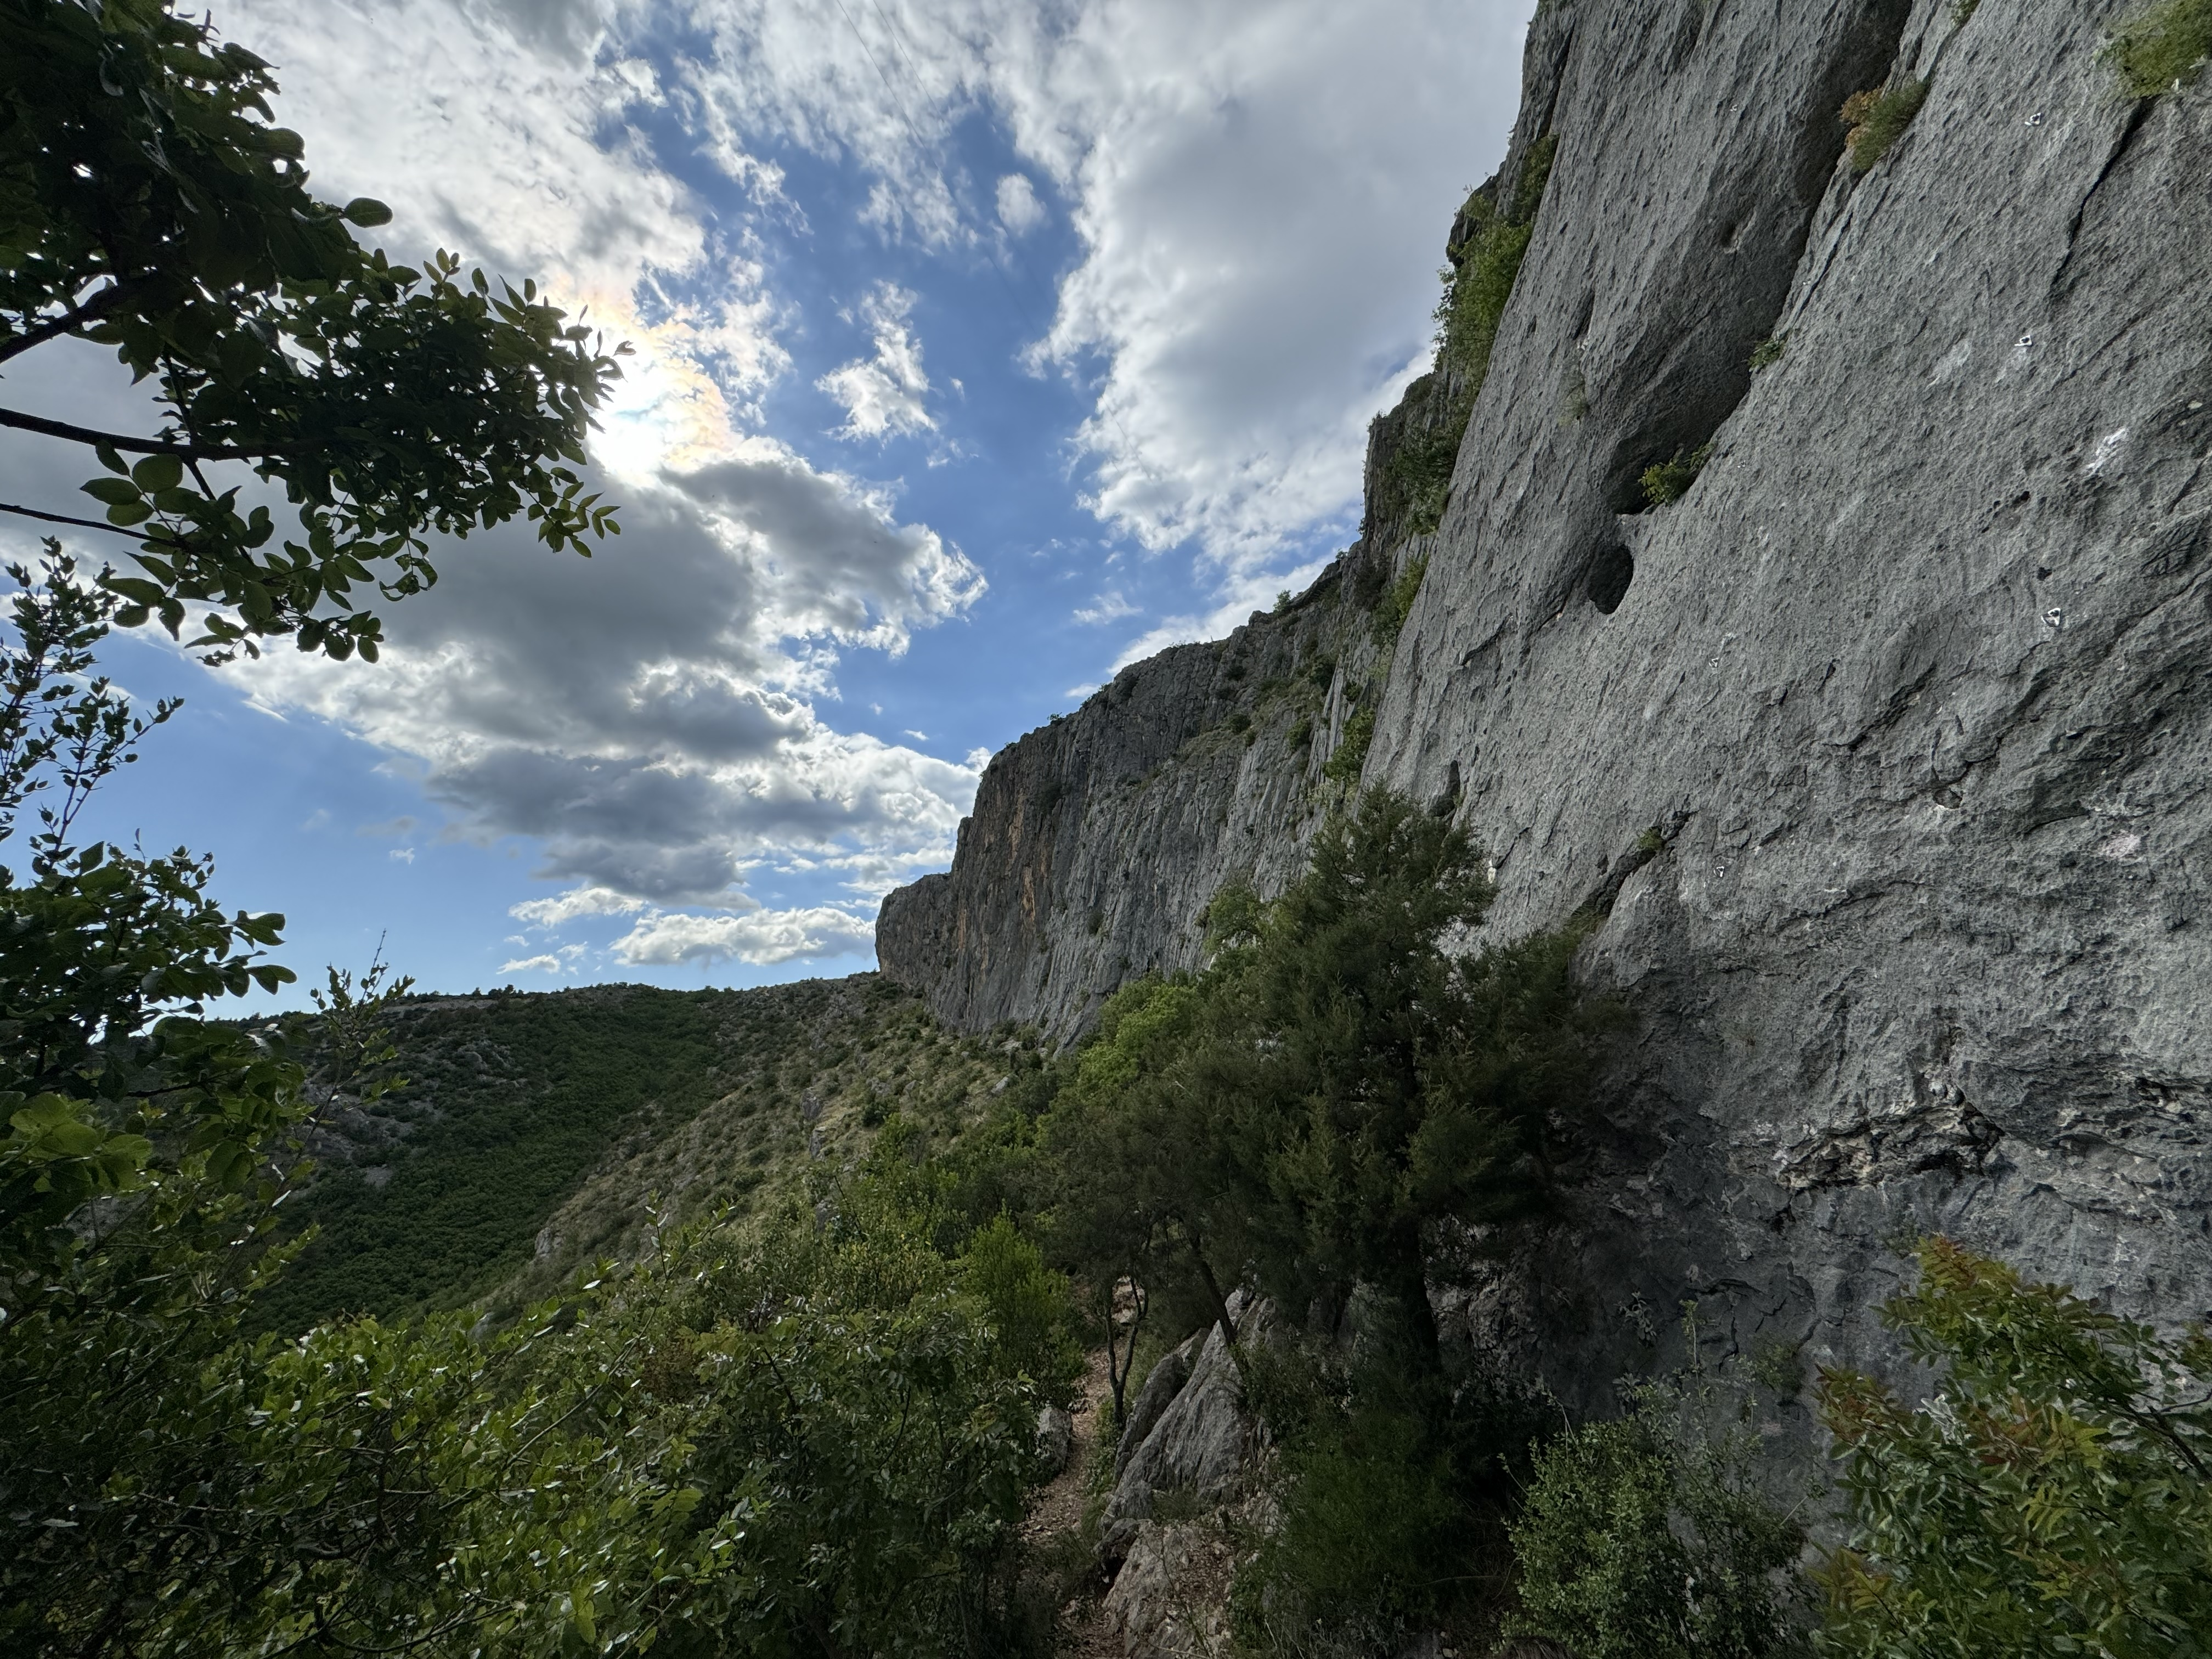
\includegraphics[width=0.8\textwidth]{images/analiza/cikola_fizicka_slika.jpg}
    \caption{Stvarna stijena na penjačkoj lokaciji Čikola sektora Osoje}
    \label{fig:cikola_fizicka_slika}
\end{figure} 

 Gledajući sliku~\ref{fig:cikola_fizicka_slika} teško je rasaznati gdje se penjač nalazi u odnosu na topo sliku i time je teško odrediti u koji penjački smjer penjač gleda. Često se traže distinktni elementi na stijeni poput velike rupe, nagle promjene u boji ili vegetacije, no ako je slika slikana iz velike udaljenost, to nije uvijek moguće. Cjelokupni proces je zahtjevan i podložan pogreškama te oduzima vrijeme koje bi se moglo iskoristiti za penjanje. Čak i uz pomoć fizičkih i digitalnih vodiča problem ostaje neriješen. Ta neefikasnost i nedostatak informacija predstavlja ključnu motivaciju za izradu sustava koji automatizira proces i pruža korisniku nedvosmislenu informaciju.

\section{Računalni vid u prepoznavanju objekata}

\subsection{Detekcija i opis značajki (engl. feature detection and description)}

\section{Uparivanje značajki (engl. feature matching)}

Nakon što se odrede SIFT značajke na obije slike, potrebno je pronaći podudaranja među njima. Proces se svodi na pronalaženje parova deskriptora koji su međusobno najsličniji u visokodimenzionalnom prostoru. Postoji nekoliko metoda za mjerenje sličnosti deskriptora.

Prva metoda je korištenje \textit{brute force} algoritma. Sličnost između dva 128-dimenzionalna SIFT deskriptora mjeri se koristeći Euklidsku udaljenost formulom
\begin{equation}
    d(d_1, d_2) = \sqrt{\sum_{i=1}^{128} (d_1[i] - d_2[i])^2}
\end{equation}
gdje su $d_1$ i $d_2$ dva 128-dimenzionalna SIFT deskriptora. Manja Euklidska udaljenost predstavlja veću sličnost između deskriptora, odnosno između lokalnih struktura slike koje oni predstavljaju.
Kada bi se uparivanje izvodilo jednostavnim pronalaskom para sa minimalnom udaljenosti došlo bi do velikog broja pogrešnih podudaranja. Zbog toga se koristi algoritam zvan Loweov test omjera~\cite{lowe2004sift}. Umjesto da se traži samo jedan, za svaki deskriptor s referentne slike pronalaze se dva najbliža susjeda na slici s kamere. Ako je omjer udaljenosti između najbližeg i drugog najbližeg susjeda manji od koeficijenta $t$, deskriptor se smatra valjanim podudaranjem. Ovo se može opisati formulom
\begin{equation}
    \frac{d(d_1, d_2)}{d(d_1, d_3)} < t
\end{equation}
gdje su $d_1$, $d_2$ i $d_3$ tri 128-dimenzionalna SIFT deskriptora, $d$ je Euklidska udaljenost, a $t$ je koeficijent koji se koristi za filtriranje pogrešnih podudaranja. Uobičajena vrijednost za prag $t$ je između 0.7 i 0.8. Ovaj test provjerava je li podudaranost nedvosmislena, odnosno ako je najbliži susjed znatno bliži od drugog onda je značajka jedistvena i podudarnost je vjerojatno ispravna. Ako to nije istina onda to ukazuje na dvosmislenost i takva podudaranost se odbacuje kao nepouzdana.

Unatoč što ovaj algoritam daje dobre rezultate, njegova vremenska komplesnost ga čini nepraktičnim za rad u stvarnom vremenu. Kako bi se ubrzao proces, često se koriste algoritmi za aproksimativnu pretragu najbližih susjeda koji se oslanjaju na efikasne strukture podataka za organizaciju visokodimezionalnih vektora. 
Jedna od takvih struktura je \textit{k-d stablo}. K-d stablo je prostorna podatkovna struktura koja rekurzivno dijeli prostor u polovične podprostore čime postiže brzu eliminaciju velikih dijelova prostora pretrage. Unatoč njenoj efikasnosti u prostorima niske dimenzionalnosti, njena primjena u visokodimenzionalnim prostorima nije učinkovita, što je problematično za 128-dimenzionalne SIFT deskriptore. 
Zato je za SIFT deskriptore bolja tehnika LSH (eng. \textit{Locality-Sensitive Hashing}) koja se oslanja na hash funkcije za brzo pronalaženje sličnih vektora u visokodimenzionalnom prostoru.
U praksi se takvi algoritmi ne implementiraju ručno već se koriste gotove biblioteke koje nude bolja rješenja. Jedna od takvih biblioteka je \textit{FLANN} (eng. \textit{Fast Library for Approximate Nearest Neighbors}) koja implementira više različitih algoritama, uključujući i k-d stablo i LSH~\cite{flannmatcher}. Bitno je navesti kako u sklopu OpenCV implementacije FLANN-a nije moguće koristiti LSH algoritam za uparivanje SIFT značajki jer je LSH algoritam implementiran samo za binarne deskriptore.
Prednost FLANN-a je u tome što može automatski odabrati najprikladniju strukturu podataka i parametre pretrage na temelju podataka i odabranih kompromisa brzine ili preciznosti. Tim algoritmima i bibliotekama se postižu veće brzine uz minimalne gubitke u preciznosti naspram \textit{brute force} algoritma.

\begin{figure}[H]
    \centering
    \includegraphics[width=0.9\textwidth]{images/racunalniVid/feature_matching.png}
    \caption{Uparivanje značajki SIFT algoritmom}
    \label{fig:uparivanje_znacajki}
\end{figure}

Na slici~\ref{fig:uparivanje_znacajki} prikazan je primjer uparivanja značajki SIFT algoritmom za referentnu sliku penjačkog smjera i sliku dobivenu s kamere mobilnog uređaja.
\section{Homografija i transformacija perspektive}

Rezultat procesa uparivanja značajki je skup parova odgovarajućih točaka između referentne slike i slike dobivene sa kamere, no taj skup gotovo uvijek sadrži i određeni broj pogrešnih podudaranja. Te pogreške nastanu zbog dvosmislenosti ili nesavršenosti SIFT deskriptora. Kako bi se uspostavila pouzdana geometrijska veza između dviju slika potrebno je pronaći matematički model koji opisuje transformaciju tih slika, ali na način koji je robustan na prisutnost tih pogrešnih parova. Takav model je homografija. 

Homografija je projektivna transformacija u 2D prostoru koja preslikava točke iz jedne ravnine u drugu. U ovom slučaju te ravnine su referentna slika i slika dobivena sa kamere. Homografija se može opisati 3x3 matričnom jednadžbom
\begin{equation}
    s *
    \begin{pmatrix}
        x' \\
        y' \\
        1
    \end{pmatrix}
    =
    \begin{pmatrix}
        h_1 & h_2 & h_3 \\
        h_4 & h_5 & h_6 \\
        h_7 & h_8 & h_9
    \end{pmatrix}
    \begin{pmatrix}
        x \\
        y \\
        1
    \end{pmatrix}
\end{equation}
gdje su $x$ i $y$ koordinate točke na referentnoj slici, a $x'$ i $y'$ koordinate točke na slici dobivenoj sa kamere. $s$ predstavlja faktor skale tj. $s$ je posljedica korištenja homogenih koordinata i predstavlja treću komponentu rezultirajućeg vektora prije normalizacije. Faktor $s$ osigurava da jednadžba vrijedi u projektivnom prostoru. Matrica $H$ je homografska matrica koja se sastoji od 9 koeficijenata, no $h_9$ je tipično postavljen na 1 što znači da matrica ima 8 stupnjeva slobode. Za njen izračun potrebno je poznavati barem 4 odgovarajuće točke na referentnoj i slici dobivenoj sa kamere, pod uvjetom da su točke nekolinearne.
Budući da za izračun homografije potrebno je samo četri para točaka, a iz procesa uparivanja dobije se znatno više parova, potrebno je odabrati najbolje parove na način da se također eliminira utjecaj pogrešnih podudaranosti. Za rješavanje ovog problema koristi se RANSAC (eng. \textit{Random Sample Consensus}) algoritam. RANSAC je iterativni algoritam koji se sastoji od sljedećih koraka. 
Prvo se nasumično odabire minimalni podskup podataka potreban za izračun homografije, odnosno četri para uparenih točaka. Na temelju tih nasumičnih točaka izračunava se preliminarna homografija $H$. Potom se ta preliminarna homografija testira na način da se ta matrica primjenjuje na sve ostale točke iz početnog seta podataka i određuje se udaljenost između izračunate točke i prave točke iz seta. Ako je ta udaljenost manja od predefiniranog praga onda se taj par smatra podudaranim s modelom. Cijeli ovaj postupak se ponavlja veliki broj puta. 
Na kraju se odabire matrica H koja je u jednoj od iteracija dobila najveći broj podudaranja s modelom. Korištenjem ovog algoritma osigurava se da pogrešne podudaranosti budu efikasno ignorirane jer se neće uklopiti u jedan konzistentan geometrijski model.

Primjer matrice homografije dobivene iz procesa uparivanja značajki prikazanog na slici~\ref{fig:uparivanje_znacajki} može izgledati ovako:

\begin{equation}
    H =
    \begin{pmatrix}
        0.6298 & 0.0750 & 412.29 \\
        0.0065 & 0.7816 & 271.09 \\
        0.000000280 & 0.0000741 & 1
    \end{pmatrix}
\end{equation}

Ova matrica $H$ transformira koordinate točaka s referentne slike penjačkog smjera na sliku dobivenu sa kamere, uzimajući u obzir rotaciju, translaciju, skaliranje i perspektivnu deformaciju. Vrijednosti u matrici su stvarni primjer dobiven iz procesa uparivanja značajki za konkretni slučaj prikazan u prethodnom poglavlju.




Kada je pronađena matrica $H$ s njom se može postići transformacija perspektive između dviju slika. Korištenjem homografije moguće je preslikati referentnu sliku linije penjačkog smjera na sliku dobivenu sa kamere koristeći OpenCV biblioteku te algoritam \textit{warpPerspective}. Kao izlaz, generira se nova slika na kojoj je sadržaj perspektivno izobličen u skladu s matricom $H$. 

\begin{figure}[H]
    \centering
    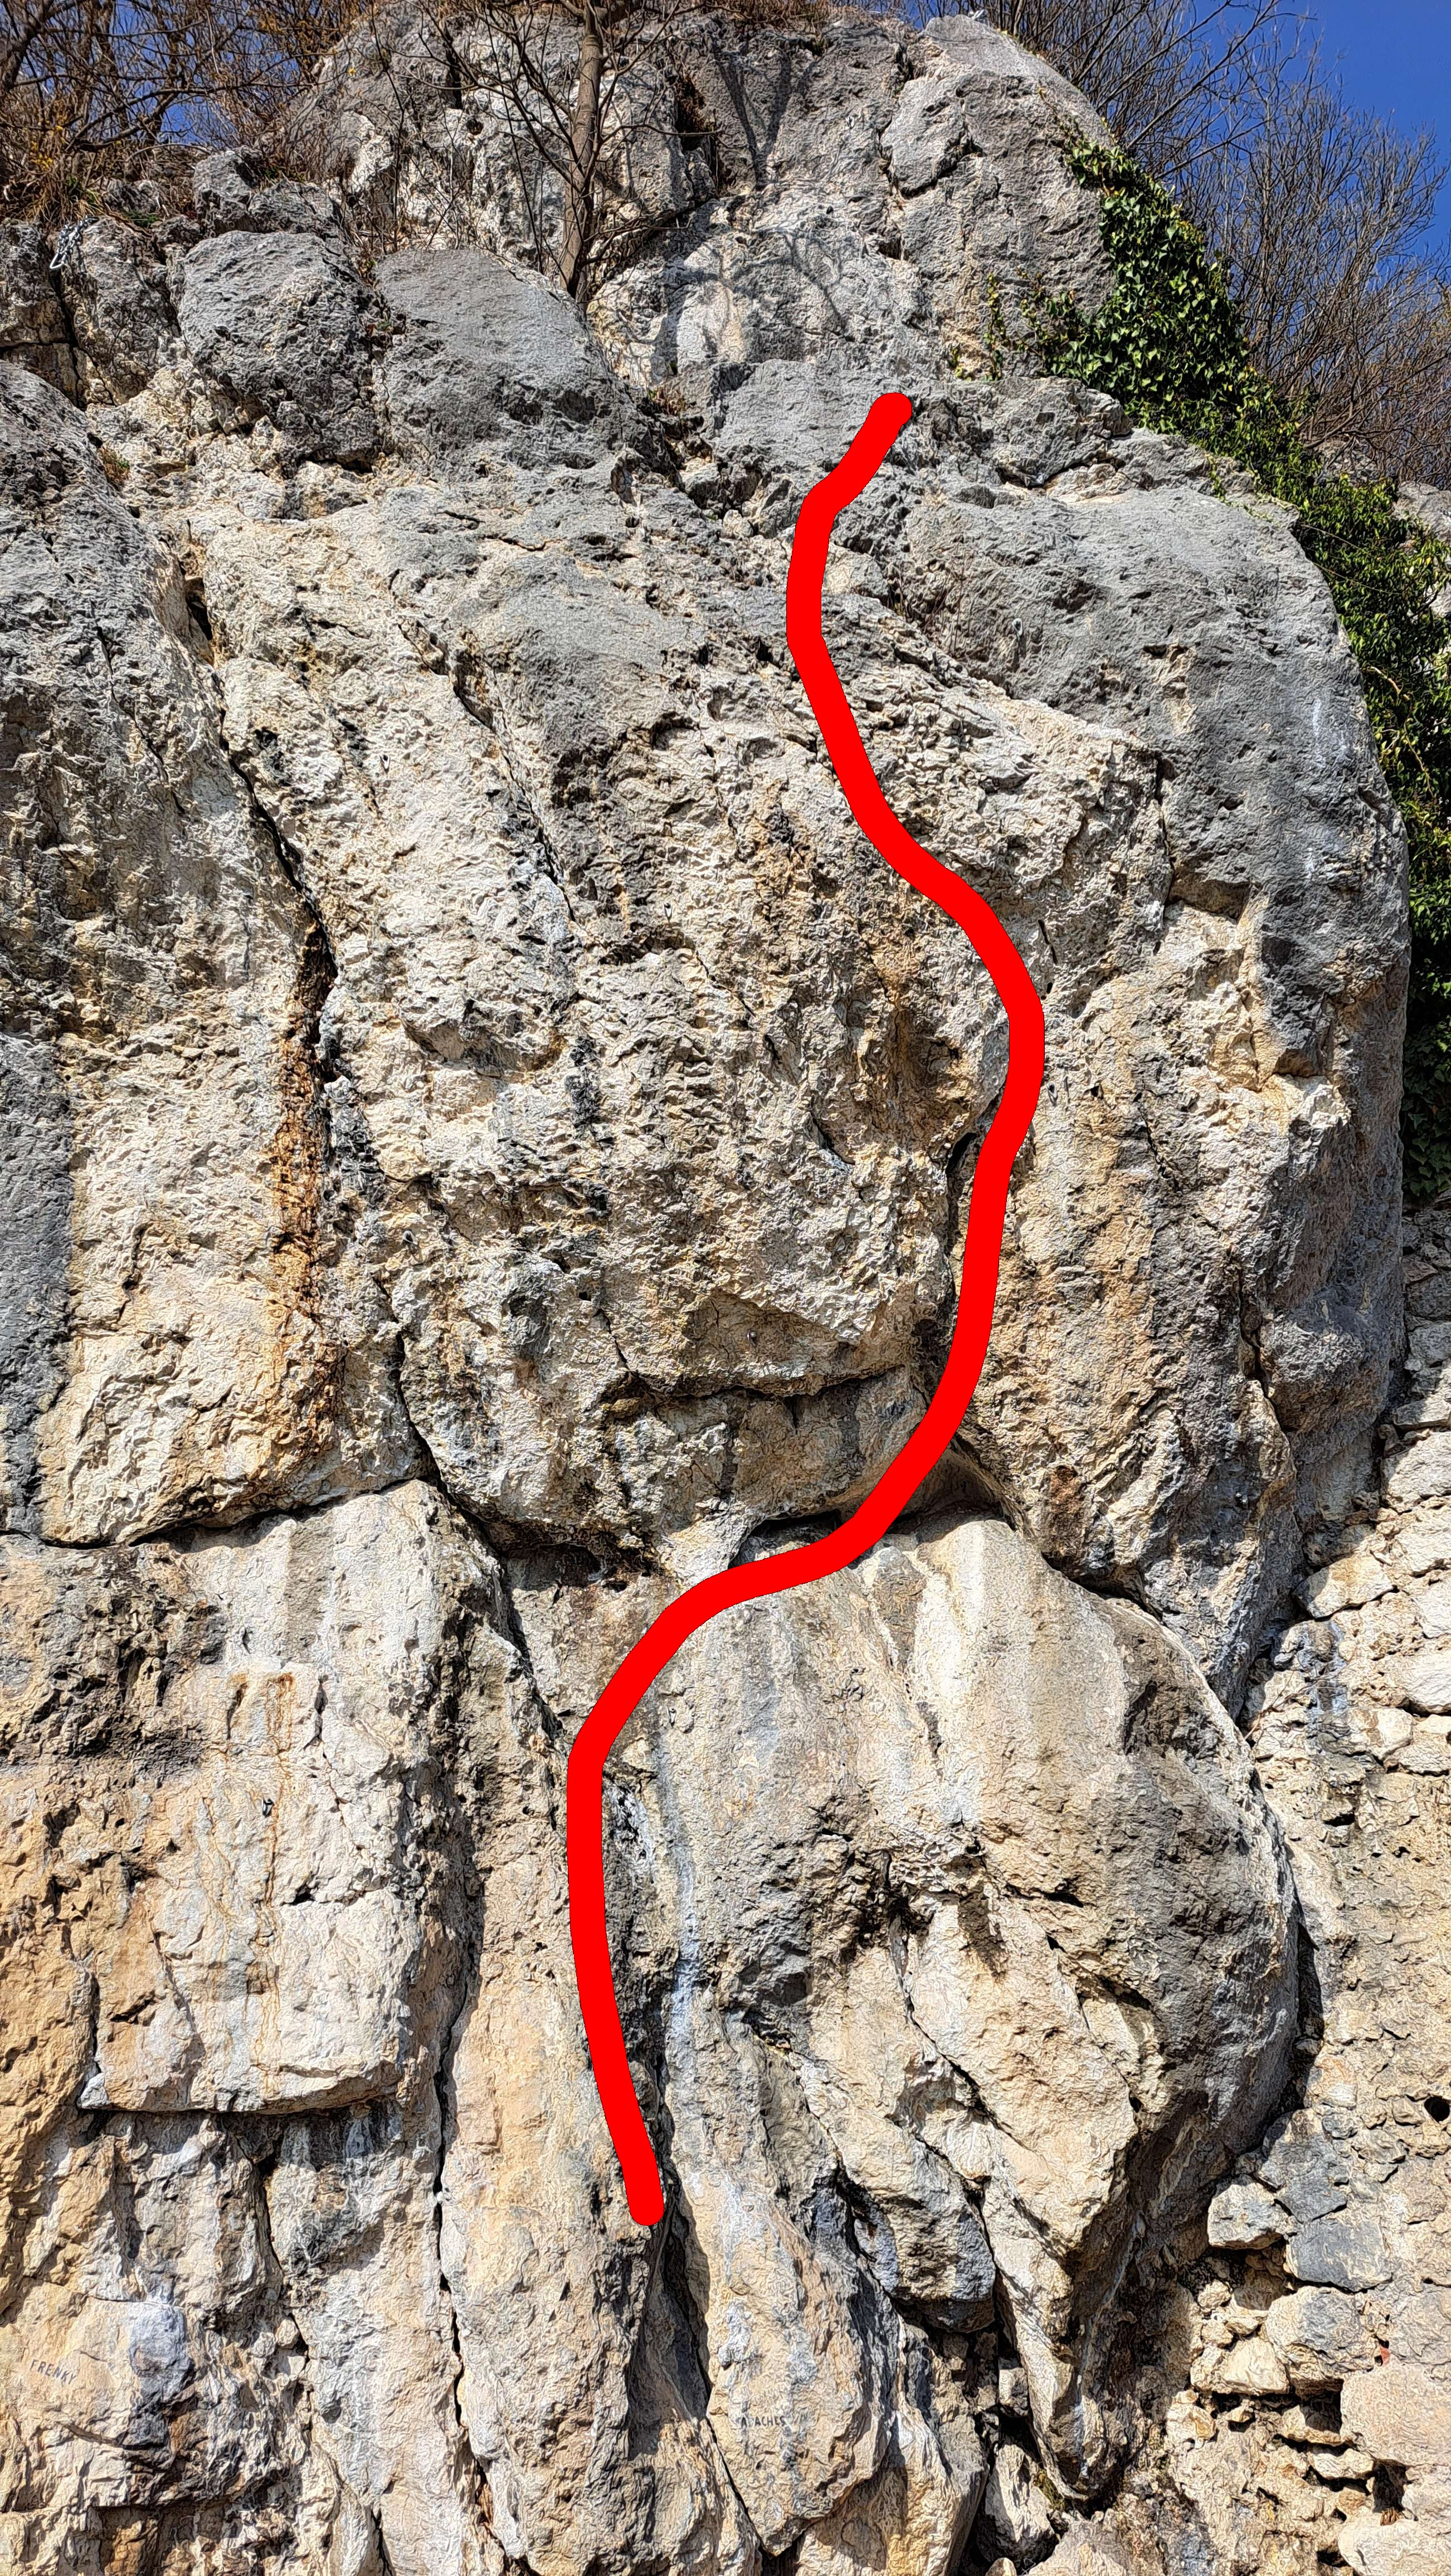
\includegraphics[width=0.4\textwidth]{images/racunalniVid/frame_with_route.jpg}
    \caption{Rezultirajuća slika transformirane linije penjačkog smjera}
    \label{fig:transformacija_perspektive}
\end{figure}

Rezultirajuća slika transformirane linije penjačkog smjera tada se može iscrtati preko slike dobivene sa kamere (slika~\ref{fig:transformacija_perspektive}). Budući da je homografija izračunata na temelju značajki sa stijene, transformirana linija će se precizno poklapati s geometrijom stijene u trenutnom pogledu kamere čime se postiže efekt proširene stvarnosti.

\section{Tehnologije za razvoj sustava}

\subsection{Razvoj za iOS platformu}
\input{sections/Analiza/subsections/backend_tehnologije.tex}
\input{sections/Analiza/subsections/web_tehnologije.tex} 